\documentclass[xcolor=table,dvipsnames,svgnames]{beamer}
% Author: alick<alick9188@gmail.com>

% This file is modified from a solution template for:

% - Giving a talk on some subject.
% - The talk is between 15min and 45min long.
% - Style is ornate.

% Copyright 2004 by Till Tantau <tantau@users.sourceforge.net>.
%
% In principle, this file can be redistributed and/or modified under
% the terms of the GNU Public License, version 2.
%
% However, this file is supposed to be a template to be modified
% for your own needs. For this reason, if you use this file as a
% template and not specifically distribute it as part of a another
% package/program, I grant the extra permission to freely copy and
% modify this file as you see fit and even to delete this copyright
% notice.

\mode<presentation>
{
  \usetheme[secheader]{Boadilla}
  \usefonttheme[onlymath]{serif}
  \setbeamercovered{transparent=5}
  \definecolor{thupurple}{HTML}{93278F}
  \definecolor{thudarkpurple}{HTML}{5C307D}
  \definecolor{thulightpurple}{HTML}{BC9BCC}
  \setbeamercolor*{structure}{fg=thupurple}
  \setbeamercolor*{palette primary}{fg=black,bg=thulightpurple}
  \setbeamercolor*{palette secondary}{fg=white,bg=thupurple}
  \setbeamercolor*{palette tertiary}{fg=white,bg=thudarkpurple}
  \setbeamercolor*{palette quaternary}{fg=white,bg=black}
}

\usepackage{mflogo} % for \MF, \MP
\usepackage{graphicx}
\graphicspath{{fig/}}
\usepackage{listings}
\usepackage{xspace}
\usepackage{amsmath}
\usepackage{wasysym} % for \smiley etc
\usepackage{calligra}
\usepackage{cclicenses} % CC symbols
\usepackage{fontspec}
\usepackage[UTF8,nofonts]{ctex}
\usepackage{hologo}
\usepackage{colortbl}
\usepackage{pstricks}
\usepackage{pst-node}
\usepackage{hyperxmp}
\hypersetup{
pdfauthor={Alick Zhao},
pdfcopyright={Copyright (C) 2015 by Alick Zhao.
Licensed under CC-BY-SA 4.0. Some rights reserved.},
pdflicenseurl={http://creativecommons.org/licenses/by-sa/4.0/},
}

% From thuthesis user guide
\makeatletter
\def\psRotation#1(#2,#3)#4{%
  \rput{#1}(#2,#3){%
    \psellipticarc[linewidth=.4pt]{->}(0,-0.1)(0.6,0.15){120}{70}
    \ifdim#1pt>\z@\rput[l]{*0}(0.675,0){#4}\else\rput[l](0.675,0){#4}\fi
  }%
}
\makeatother

% For tipa to work.
\newfontfamily\useTIPAfont{Times New Roman}

% xeCJK conf setup
\punctstyle{kaiming}
\renewcommand\CJKfamilydefault{\CJKsfdefault} % for slides

\setCJKmainfont[BoldFont={SimHei},
ItalicFont={KaiTi}]{SimSun}
\setCJKsansfont{WenQuanYi Micro Hei}
\setCJKmonofont{WenQuanYi Micro Hei Mono}

\setCJKfamilyfont{zhsong}{SimSun}
\setCJKfamilyfont{zhhei}{SimHei}
\setCJKfamilyfont{zhkai}{KaiTi}

\newcommand*{\songti}{\CJKfamily{zhsong}} % 宋体
\newcommand*{\heiti}{\CJKfamily{zhhei}}   % 黑体
\newcommand*{\kaishu}{\CJKfamily{zhkai}}  % 楷书

%\renewcommand\tablename{表格}

\newcommand{\BibTeX}{\hologo{BibTeX}}
\newcommand{\XeTeX}{\hologo{XeTeX}}
\newcommand{\pdfTeX}{\hologo{pdfTeX}}
\newcommand{\beamer}{\textsc{beamer}}
\def\TeXLive{\TeX{} Live\xspace}
\let\TL=\TeXLive
\newcommand{\ThuThesis}{\textsc{ThuThesis}\xspace}

% From thuthesis user guide.
\def\cmd#1{\texttt{\color{DarkBlue}\footnotesize $\backslash$#1}}
\def\env#1{\texttt{\color{DarkBlue}\footnotesize #1}}
\def\cmdxmp#1#2#3{\small{\texttt{\color{DarkBlue}$\backslash$#1}\{#2\}\hspace{1em}\\ $\Rightarrow$\hspace{1em} {#3}\par\vskip1em}}

%\includeonlyframes{current}

\title
{如何使用 \LaTeX 排版论文}

\author[alick] % (optional, use only with lots of authors)
{赵涛\\ \texttt{alick9188@gmail.com}}

\institute[GitHub] % (optional, but mostly needed)
{
  清华大学电子系网络融合实验室
}
% - Use the \inst command only if there are several affiliations.
% - Keep it simple, no one is interested in your street address.

\date[图书馆专题培训讲座] % (optional)
{\today}

\subject{LaTeX, paper, ThuThesis}

% Delete this, if you do not want the table of contents to pop up at
% the beginning of each subsection:
\AtBeginSubsection[]
{
  \begin{frame}<beamer>{目录}
    \tableofcontents[currentsection,currentsubsection]
  \end{frame}
}


% If you wish to uncover everything in a step-wise fashion, uncomment
% the following command:

%\beamerdefaultoverlayspecification{<+->}

\lstset{basicstyle=\footnotesize\ttfamily,breaklines=true}
\hypersetup{
%pdfpagemode=FullScreen,
}

\logo{
\includegraphics[height=.15\textheight]{libicon.jpg}}

\begin{document}

\begin{frame}
  \titlepage
\end{frame}

\begin{frame}{目录}
  \tableofcontents
  % You might wish to add the option [pausesections]
\end{frame}


% Since this a solution template for a generic talk, very little can
% be said about how it should be structured. However, the talk length
% of between 15min and 45min and the theme suggest that you stick to
% the following rules:

% - Exactly two or three sections (other than the summary).
% - At *most* three subsections per section.
% - Talk about 30s to 2min per frame. So there should be between about
%   15 and 30 frames, all told.

\section{简介}

\subsection{\TeX 与 \LaTeX}

\begin{frame}[fragile]{\TeX 与 \LaTeX}
  % TODO: photo of Knuth & Lamport
  \begin{itemize}
    \item \TeX: $\tau\varepsilon\chi$ (\textipa{/'tEx/},
      \textipa{/'tEk/})
      \begin{itemize}
         % FIXME: E/e?
         \item 生成精美图书的排版系统
         \item 最初由 高德纳 (Donald E.~Knuth) 于 1978 年开发
           %\item 最新版本为 \TeX\ 3.14159265
         \item 漂亮、美观、稳定、通用
         \item 尤其擅长数学公式排版
       \end{itemize}
    \item \LaTeX\ (\textipa{/'la:tEx/}, \textipa{/'leItEk/})
      \begin{itemize}
        \item Leslie Lamport 开发 \LaTeX 降低使用门槛
        \item 极其丰富的宏包,提供扩展功能
        \item 广泛用于学术界,期刊会议论文模板
        \item 大学学位论文模板,如 \ThuThesis
      \end{itemize}
  \end{itemize}
\end{frame}

\begin{frame}{和 Word 对比}
  \begin{table}[h]
    \centering
    \rowcolors[]{1}{blue!20}{blue!10}
    \begin{tabular}{c|c}
      Word & \LaTeX \\
      \hline
      字处理工具 & 专业排版软件 \\
      容易上手,简单直观 & 容易上手 \\
      所见即所得 & 所见即所想,所想即所得 \\
      高级功能不易掌握 & 进阶难,但一般用不到 \\
      处理长文档需要丰富经验 & 和短文档处理基本无异 \\
      花费大量时间调格式'' & 无需担心格式,专心作者内容 \\
      公式排版差强人意 & 尤其擅长公式排版 \\
      二进制格式,兼容性差 & 文本文件,易读、稳定 \\
      付费商业许可 & 自由免费使用 \\
    \end{tabular}
  \end{table}
\end{frame}

\begin{frame}{\TeX{}排版举例:公式}
  \begin{exampleblock}{无编号公式}
  \begin{equation*}
    \mathcal{F}(\xi)=\int_{-\infty}^{\infty}
    f(x)\mathrm{e}^{-\mathrm{j}2\pi \xi x}\,\mathrm{d}x
  \end{equation*}
  \end{exampleblock}
  \begin{exampleblock}{多行多列公式}
    % Taken from Mathmode.tex
\begin{align}
	y & =d & z & =1\\
	y & =cx+d & z & =x+1\\
	y_{12} & =bx^{2}+cx+d & z & =x^{2}+x+1\nonumber \\
	y(x) & =ax^{3}+bx^{2}+cx+d & z & =x^{3}+x^{2}+x+1
\end{align}
  \end{exampleblock}
\end{frame}

\begin{frame}{\TeX{}排版举例:公式}
  \begin{exampleblock}{编号多行公式}
    % Taken from Mathmode.tex
  \begin{multline}
    A=\lim_{n\rightarrow\infty}\Delta x\left(a^{2}+\left(a^{2}+2a\Delta x+\left(\Delta x\right)^{2}\right)\right.\label{eq:reset}\\
    +\left(a^{2}+2\cdot2a\Delta x+2^{2}\left(\Delta x\right)^{2}\right)\\
    +\left(a^{2}+2\cdot3a\Delta x+3^{2}\left(\Delta x\right)^{2}\right)\\
    +\ldots\\
    \left.+\left(a^{2}+2\cdot(n-1)a\Delta x+(n-1)^{2}\left(\Delta x\right)^{2}\right)\right)\\
    =\frac{1}{3}\left(b^{3}-a^{3}\right)
  \end{multline}
  \end{exampleblock}
\end{frame}

\begin{frame}{\TeX{}排版举例:图形}
  \begin{minipage}[c]{0.3\linewidth}
\psset{unit=0.8cm}
  \begin{pspicture}(-1.75,-3)(3.25,4)
\psline[linewidth=0.25pt](0,0)(0,4)
\rput[tl]{0}(0.2,2){$\vec e_z$}
\rput[tr]{0}(-0.9,1.4){$\vec e$}
\rput[tl]{0}(2.8,-1.1){$\vec C_{ptm{ext}}$}
\rput[br]{0}(-0.3,2.1){$\theta$}
\rput{25}(0,0){%
  \psframe[fillstyle=solid,fillcolor=lightgray,linewidth=.8pt](-0.1,-3.2)(0.1,0)}
\rput{25}(0,0){%
  \psellipse[fillstyle=solid,fillcolor=yellow,linewidth=3pt](0,0)(1.5,0.5)}
\rput{25}(0,0){%
  \psframe[fillstyle=solid,fillcolor=lightgray,linewidth=.8pt](-0.1,0)(0.1,3.2)}
\rput{25}(0,0){\psline[linecolor=red,linewidth=1.5pt]{->}(0,0)(0.,2)}
\psRotation{0}(0,3.5){$\dot\phi$}
\psRotation{25}(-1.2,2.6){$\dot\psi$}
\psline[linecolor=red,linewidth=1.25pt]{->}(0,0)(0,2)
\psline[linecolor=red,linewidth=1.25pt]{->}(0,0)(3,-1)
\psline[linecolor=red,linewidth=1.25pt]{->}(0,0)(2.85,-0.95)
\psarc{->}{2.1}{90}{112.5}
\rput[bl](.1,.01){C}
\end{pspicture}
  \end{minipage}\hspace{1cm}
\begin{minipage}[t]{0.5\linewidth}
\psset{unit=0.3cm}
\begin{pspicture}(1,2)(18,14)
%\psgrid[gridcolor=lightgray,subgriddiv=0,subgridcolor=lightgray]
%
\psline[linewidth=1pt,linecolor=black](6,0.5)(6,14)
\psline[linewidth=1pt,linecolor=black](1,8.5)(6,7)
\psline[linewidth=1pt,linecolor=black](1.5,5.5)(11,8.5)
%
\rput(17,3){$x$}
\rput(5.5,13){$y$}
\rput(10.5,8.75){$z$}
\rput(11,7.1){$\vec{r}$}
%
\psline[linewidth=1.5pt,linecolor=black]{<->}(6,7)(6,11.25)
\rput(5.35,9.4){$R$}
\psline[linewidth=1.5pt,linecolor=Green]{->}(6.5,12)(4.75,12)
\rput(7.5,12.8){ $I d\vec{l}$}
%
\psellipse[doubleline=true,doublecolor=yellow,doublesep=3pt,linecolor=blue](6,7)(3,4.5)
\psline[linewidth=1pt,linecolor=black](6,7)(17.5,3.5)
\psline[linewidth=1.5pt,linecolor=black]{->}(6,11.38)(11.95,5.225)
%
\psarc[linewidth=1.5pt,linecolor=gray](6,8){3.4}{85}{95}
%
\psline[linewidth=1.5pt,linecolor=gray]{->}(12,5.15)(12,8.15)
\psline[linewidth=1.5pt,linecolor=black]{->}(12,5.15)(15,7.25)
\psline[linewidth=1.5pt,linecolor=gray]{->}(12,5.15)(15,4.25)
%
\psline[linewidth=1pt,linecolor=black](12,8.15)(15,7.25)(15,4.25)
%
\Cnode*[linecolor=black,radius=0.1cm](12,5.15){a}
\rput(11.5,4.5){ $P$}
%
\rput(12.5,8.9){$dB_y$}
\rput(14.5,3.4){$dB_x$}
\rput(15.5,8){ $d \boldmath{\vec{B}}$}
%
\psarc[linewidth=1pt]{<->}(12,5){5.5}{133}{161}
\rput(7.2,8.5){ $\theta$}
\end{pspicture}
\medskip

%\hspace{2cm}
\begin{figure}[h]
  \centering
  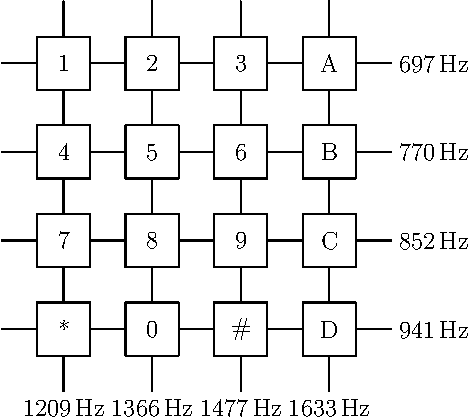
\includegraphics[height=.33\textheight]{dtmf.pdf}
\end{figure}
\end{minipage}
\end{frame}

\begin{frame}{\TeX{}排版举例:文档}
  \begin{columns}
    \begin{column}{.45\textwidth}
      \begin{figure}[h]
        \centering
        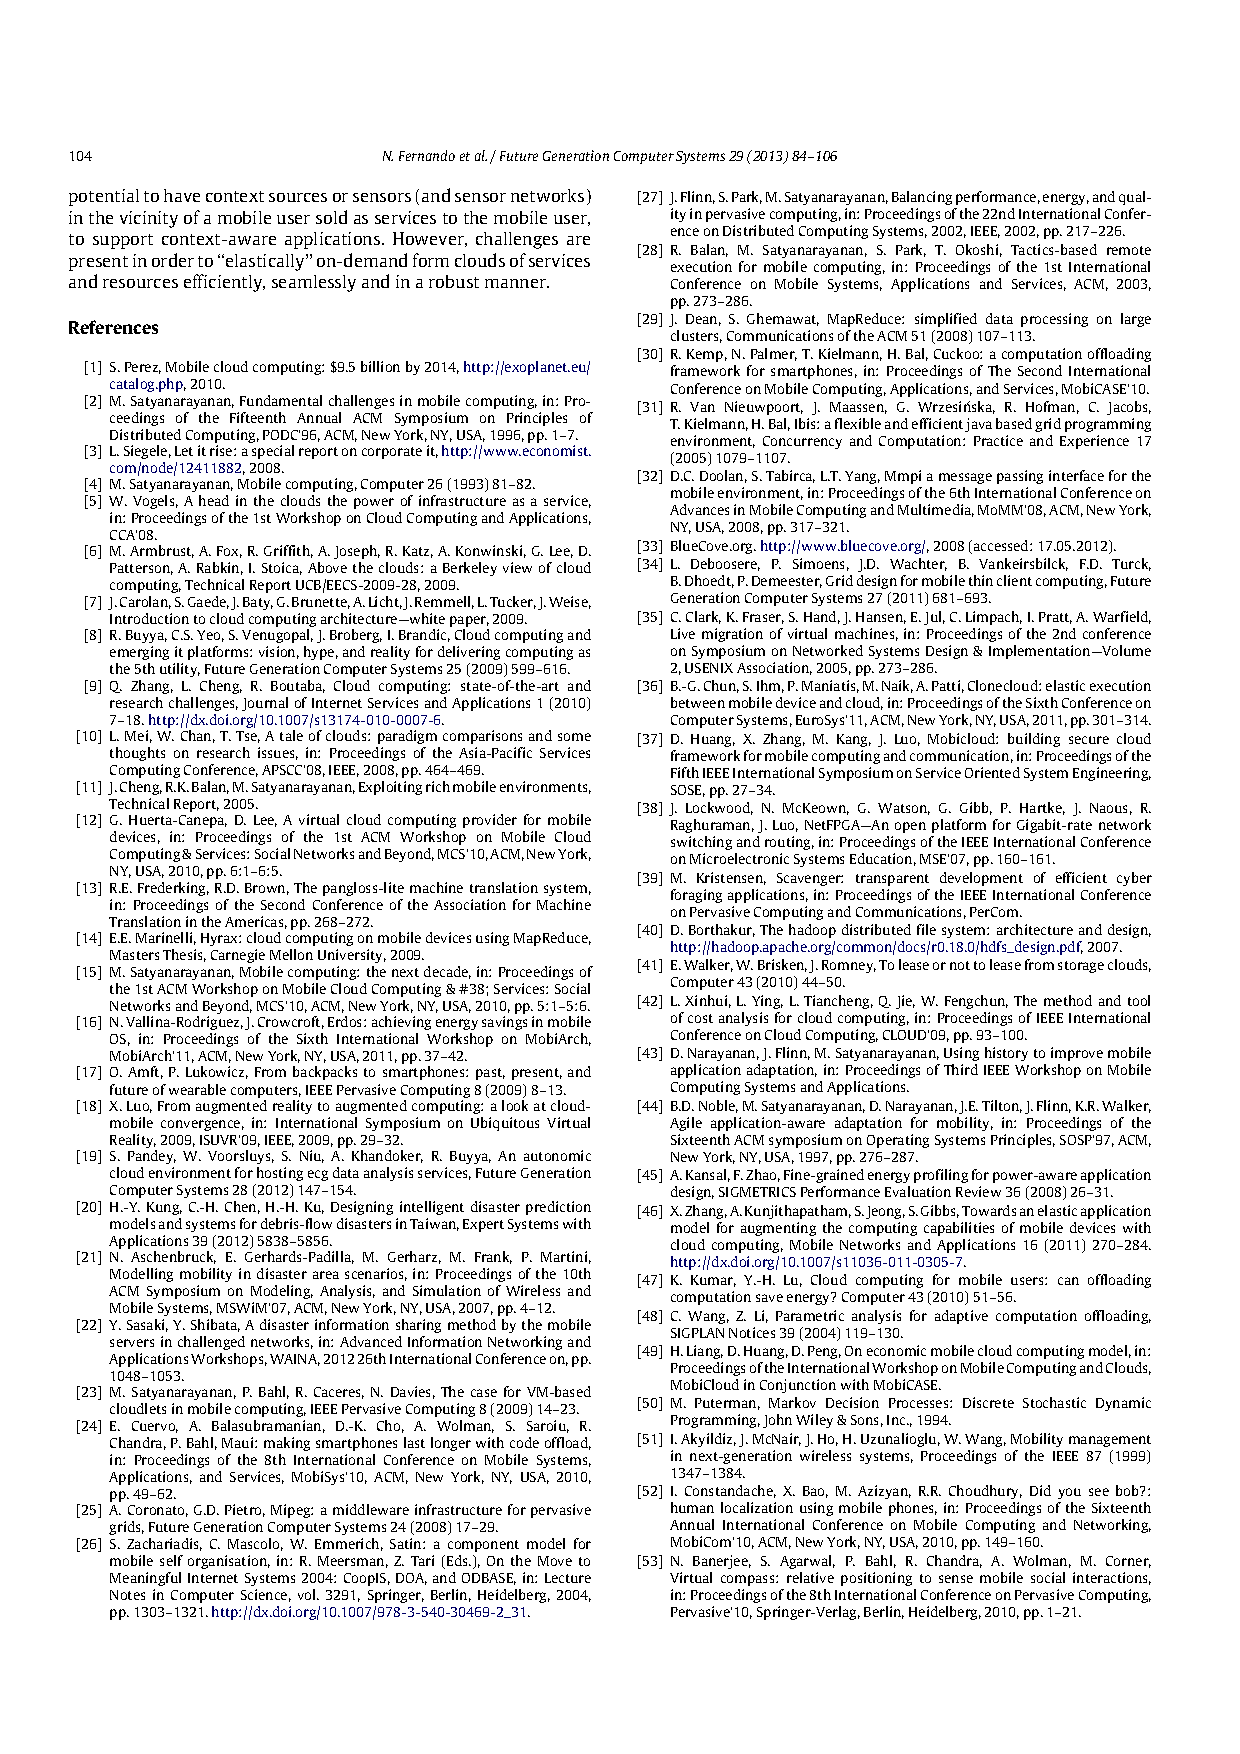
\includegraphics[width=\textwidth]{references.pdf}
      \end{figure}
    \end{column}
    \begin{column}{.45\textwidth}
      \begin{figure}[h]
        \centering
        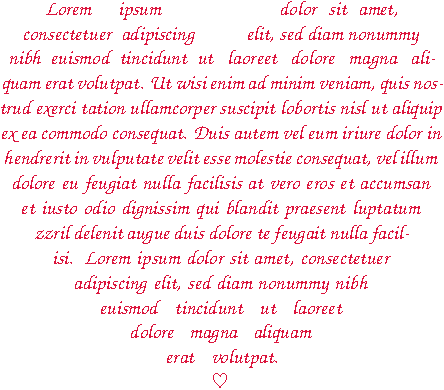
\includegraphics[width=\textwidth]{shapepar.pdf}
      \end{figure}
    \end{column}
  \end{columns}
\end{frame}

\begin{frame}{\TeX{}排版举例:幻灯片}
  \begin{columns}
    \begin{column}{.45\textwidth}
      \begin{figure}[h]
        \centering
        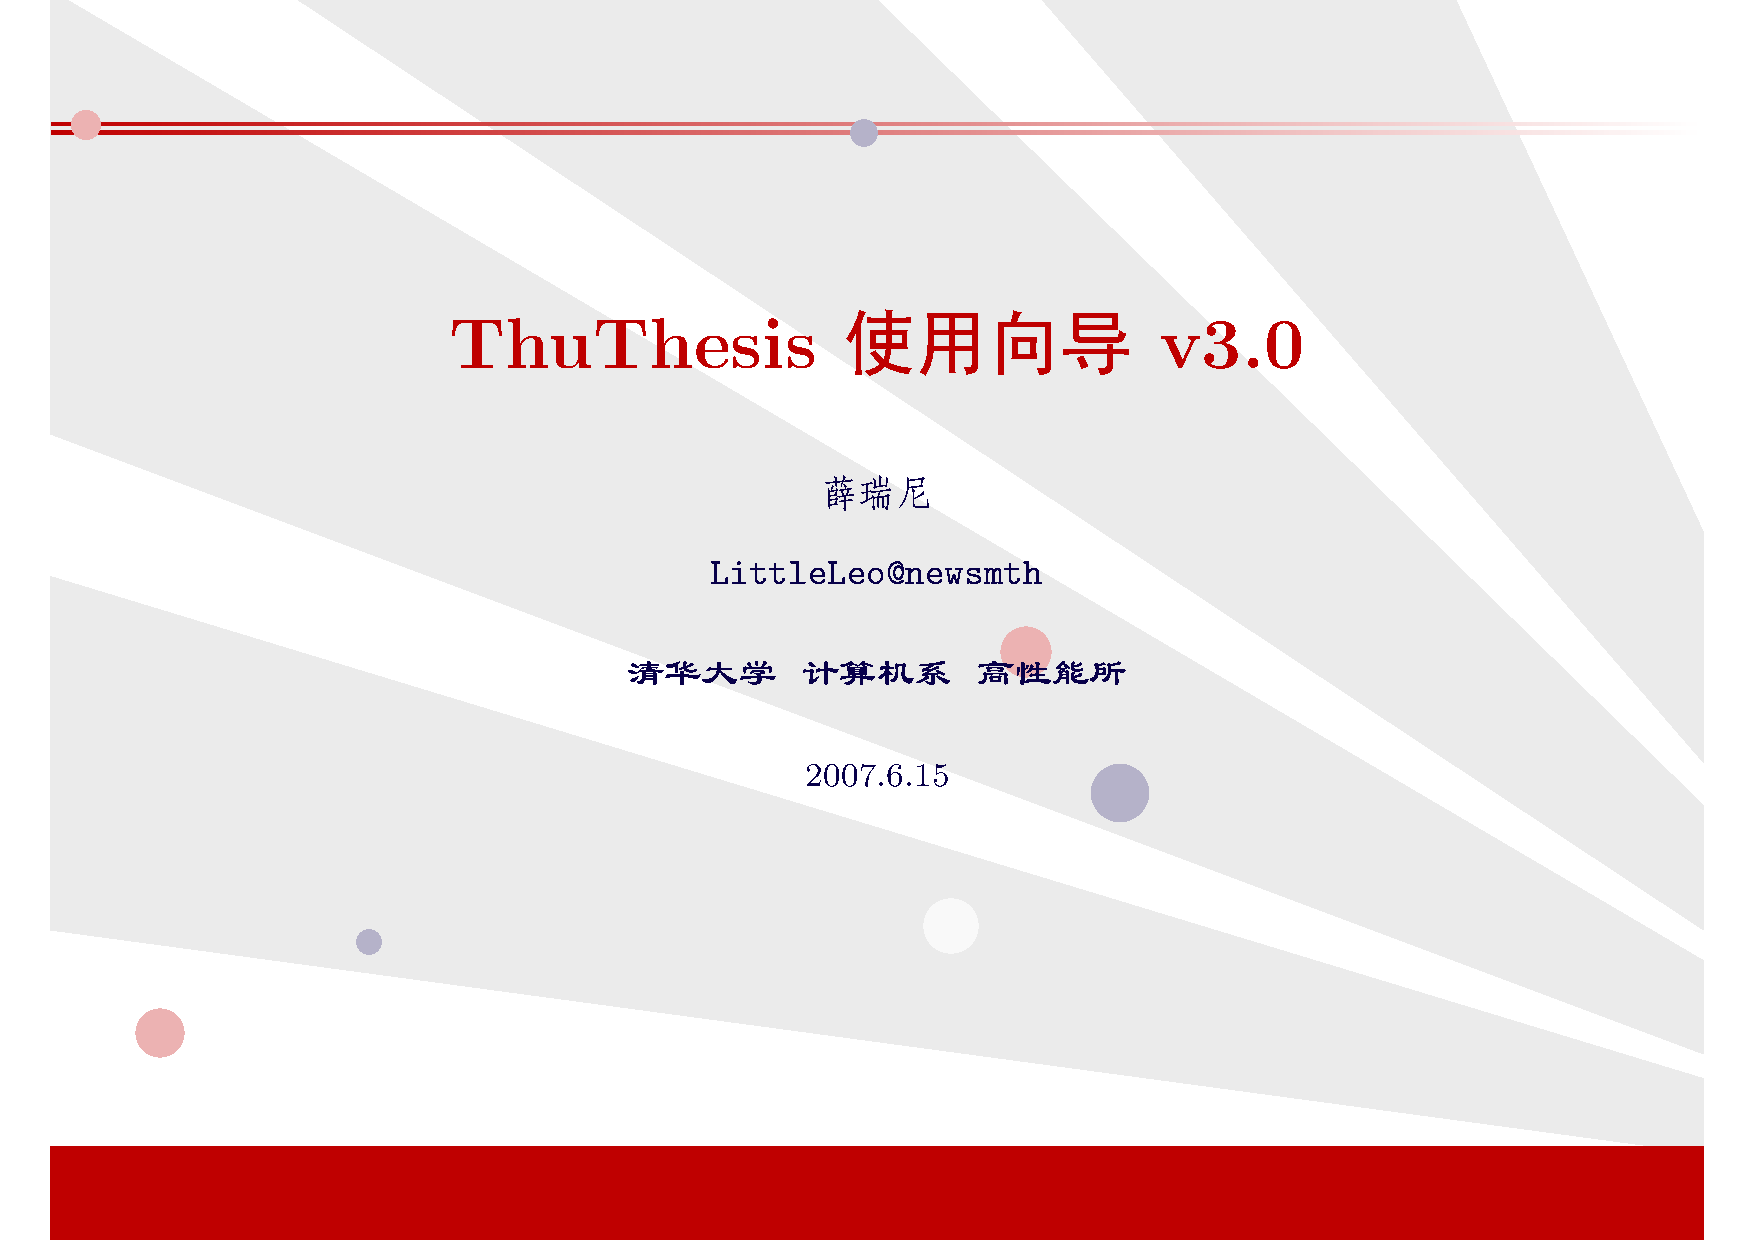
\includegraphics[width=\textwidth]{slides-powerdot.pdf}
      \end{figure}
    \end{column}
    \begin{column}{.45\textwidth}
      \begin{figure}[h]
        \centering
        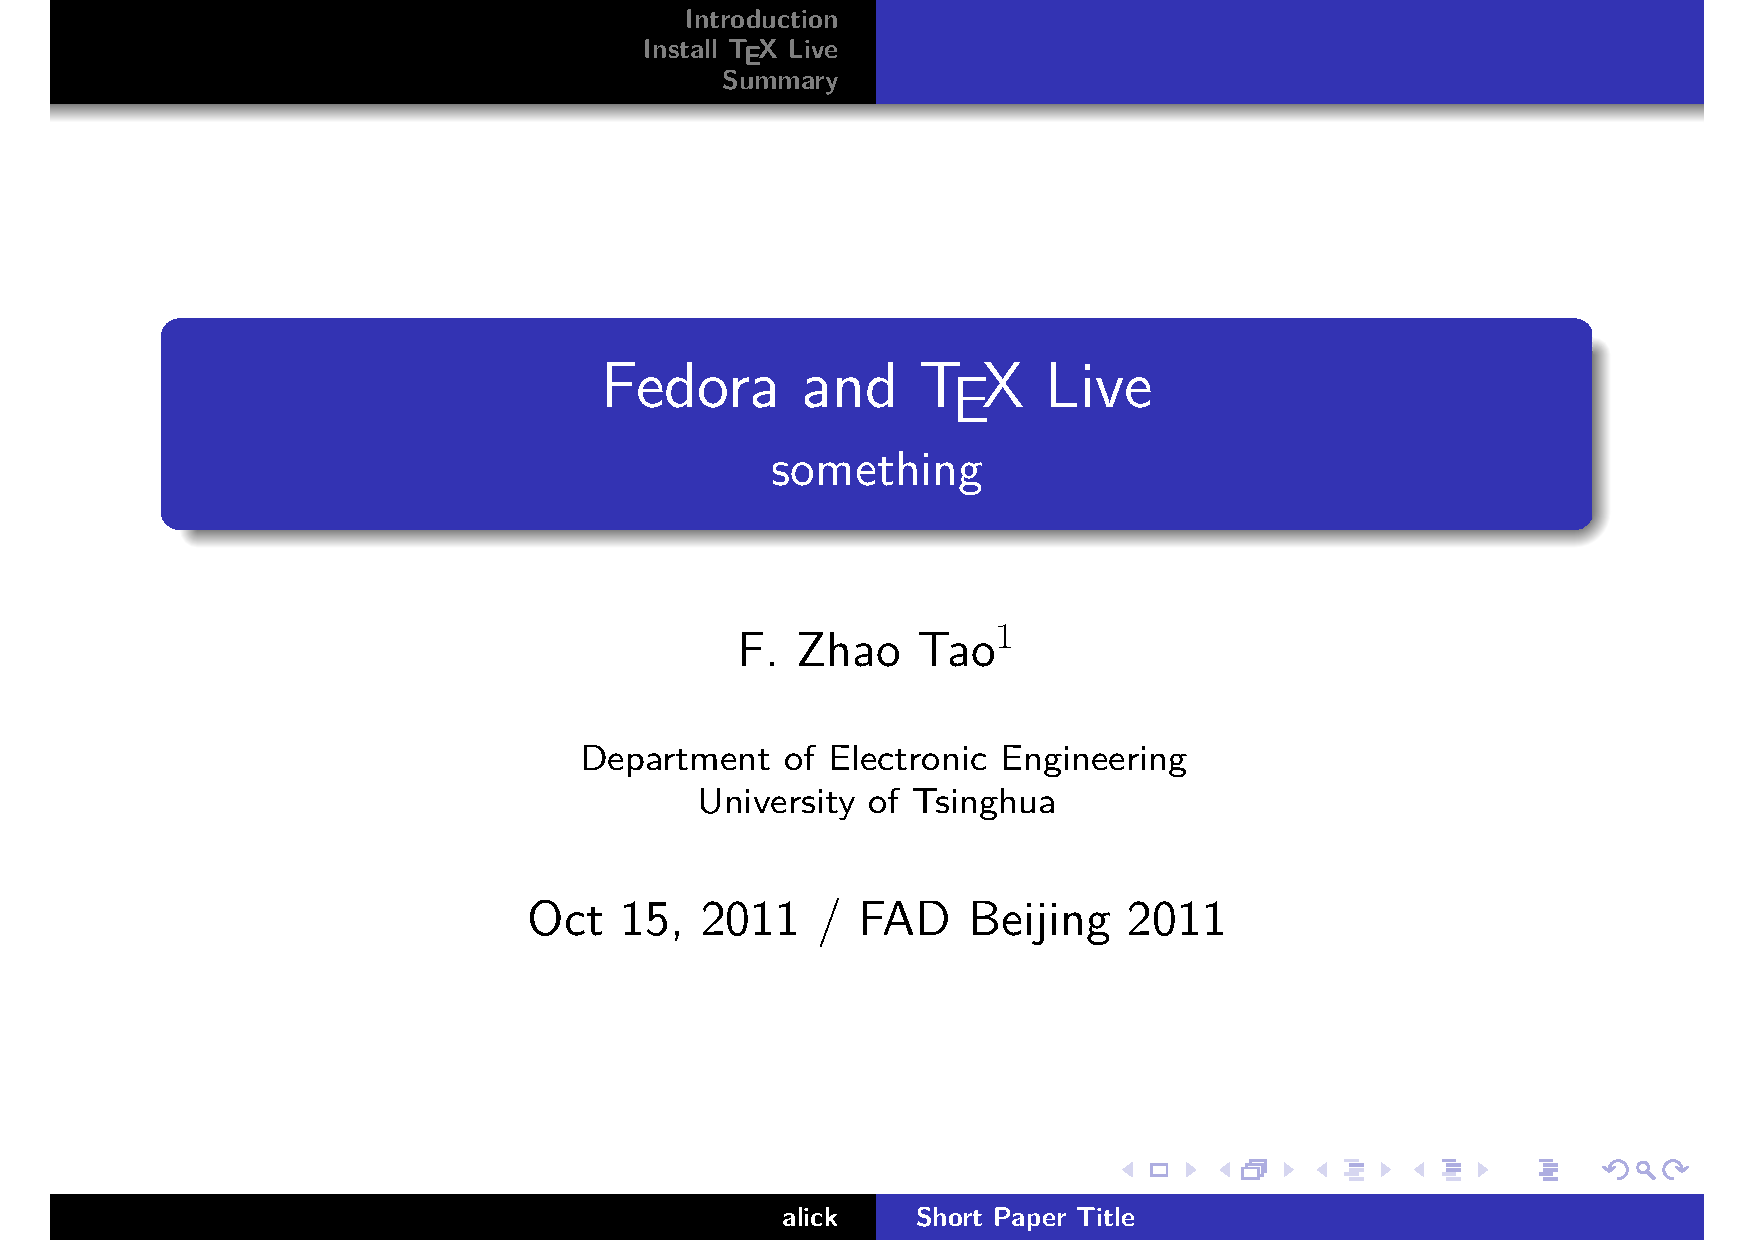
\includegraphics[width=\textwidth]{slides-beamer.pdf}
      \end{figure}
    \end{column}
  \end{columns}
\end{frame}

\subsection{安装}

\begin{frame}{如何安装 \hologo{(La)TeX}?}
  \begin{itemize}
    \item \TeX{}发行版(Distro)
      \begin{itemize}
        \item \TeX{}实用工具大集合:引擎、宏包、文档等
        \item 常见\TeX{}发行版:CTeX 套装、\hologo{MiKTeX}、\alert{\TL}
      \end{itemize}
    \item \TL
      \begin{itemize}
        \item 跨平台:Windows, Linux, Mac OS X (Mac\TeX)
        \item 每年一个新版本发布,当前 \TL 2014
      \end{itemize}
  \end{itemize}
\end{frame}

\begin{frame}[fragile]
  \frametitle{网络安装}
  \begin{itemize}
    \item 从 CTAN 镜像下载安装包(.exe 或 .zip 或 .tar.gz 格式)
(和相应的校验文件,以 .sha256 结尾)
\begin{itemize} % several mirror url
  \item 清华镜像 \url{http://mirrors.tuna.tsinghua.edu.cn/CTAN/systems/texlive/tlnet/}
  \item CTeX 镜像 \url{http://ftp.ctex.org/mirrors/CTAN/systems/texlive/tlnet/}
  \item 更多可见 \url{http://mirror.ctan.org/README.mirrors}
\end{itemize}

\item 可选步骤:校验安装包
\begin{lstlisting}
$ LANG=C sha256sum --check install-tl-unx.tar.gz.sha256
install-tl-unx.tar.gz: OK
\end{lstlisting}

  \end{itemize}
\end{frame}

\begin{frame}[fragile]
  \frametitle{网络安装}
  \begin{itemize}
    \item Windows
      \begin{itemize}
        \item 双击下载的安装程序
        \item 切换默认仓库为国内镜像:加速网络下载
      \end{itemize}
    \item Linux
      \begin{itemize}
        \item 图形安装界面需要 Perl Tk 模块:\texttt{yum install
          perl-Tk}
      \begin{lstlisting}
sudo mkdir /usr/local/texlive
sudo chown yourname:yourname /usr/local/texlive
./install-tl -gui -repository http://mirrors.tuna.tsinghua.edu.cn/CTAN/systems/texlive/tlnet/
      \end{lstlisting}
      \end{itemize}
\item 截图\dots
\end{itemize}
\end{frame}

\begin{frame}
  \begin{figure}[h]
  \centering
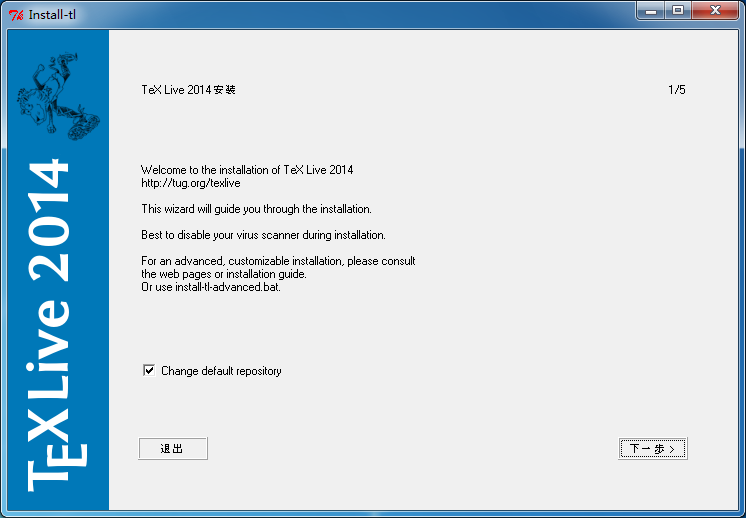
\includegraphics[scale=0.5]{simple1.png}
  \end{figure}
\end{frame}

\begin{frame}
  \begin{figure}[h]
  \centering
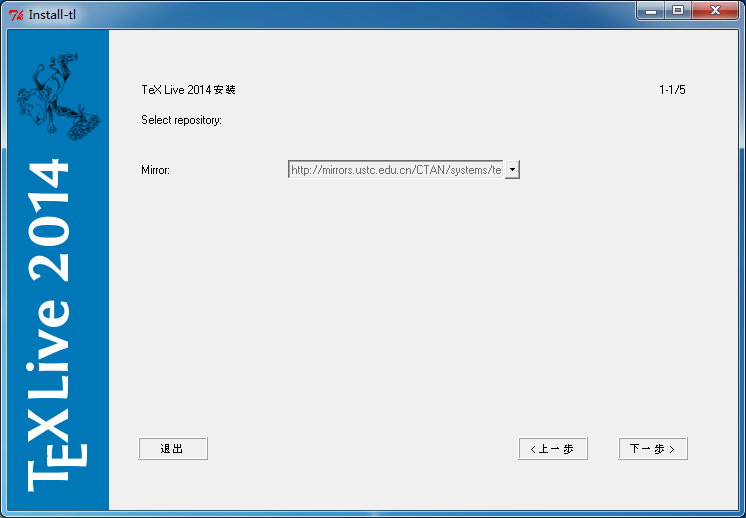
\includegraphics[scale=0.5]{simple2-ustc.png}
  \end{figure}
\end{frame}

\begin{frame}
  \begin{figure}[h]
  \centering
  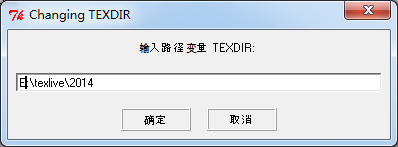
\includegraphics[height=.25\textheight]{simple3-dir.png}\\
  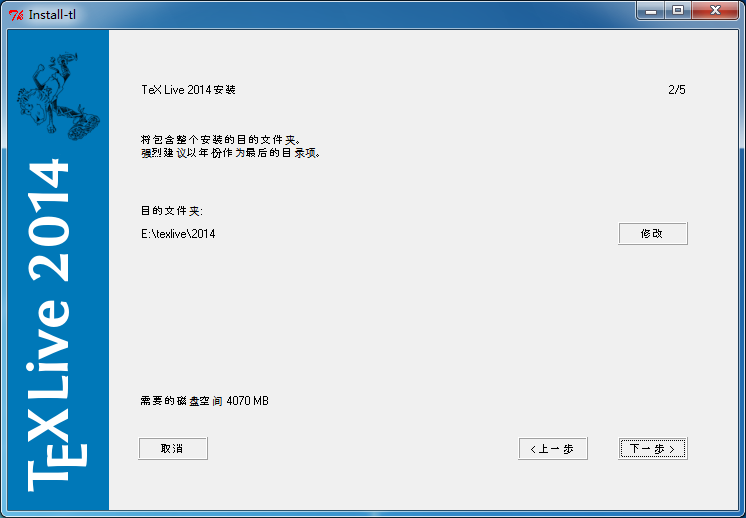
\includegraphics[scale=0.4]{simple4.png}
  \end{figure}
\end{frame}

\begin{frame}
  \begin{figure}[h]
  \centering
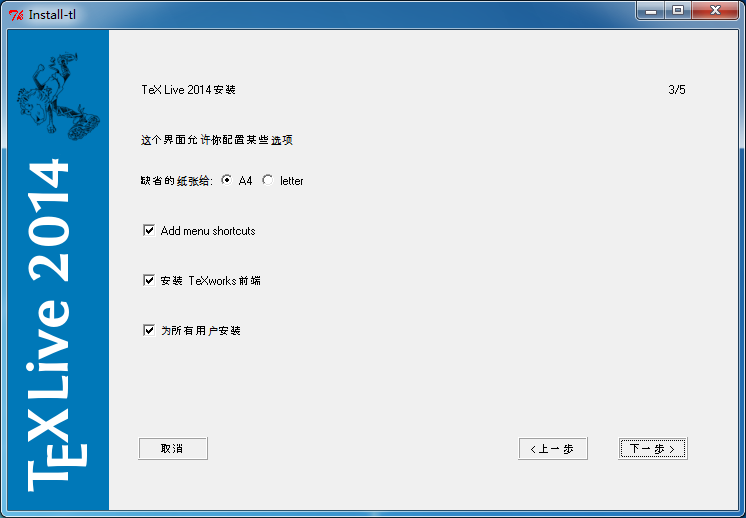
\includegraphics[scale=0.5]{simple5-opt.png}
  \end{figure}
\end{frame}

% 准备安装

\begin{frame}
  \begin{figure}[h]
  \centering
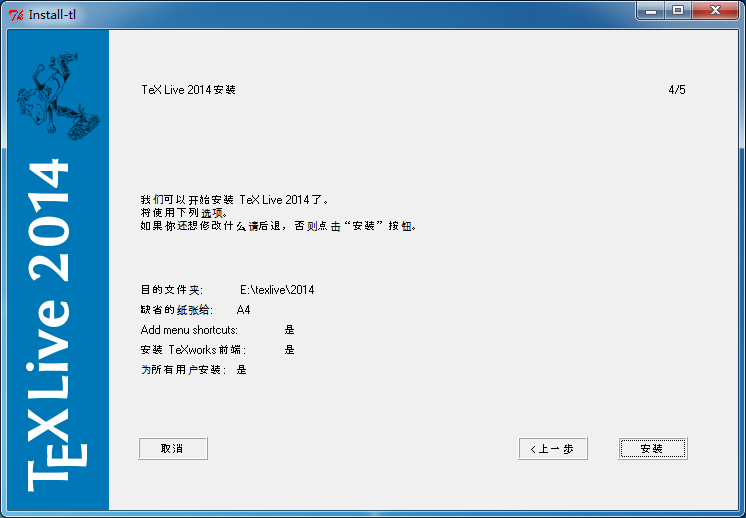
\includegraphics[scale=0.5]{simple6-preinstall.png}
  \end{figure}
\end{frame}

% 安装进行中
\begin{frame}
  \begin{figure}[h]
  \centering
  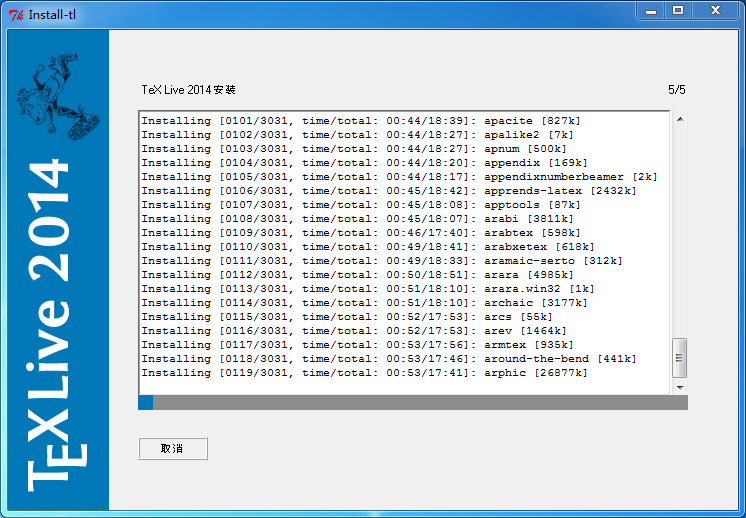
\includegraphics[scale=0.5]{simple7-installing.png}
  \end{figure}
\end{frame}

% 安装后期
\begin{frame}
  \begin{figure}[h]
  \centering
  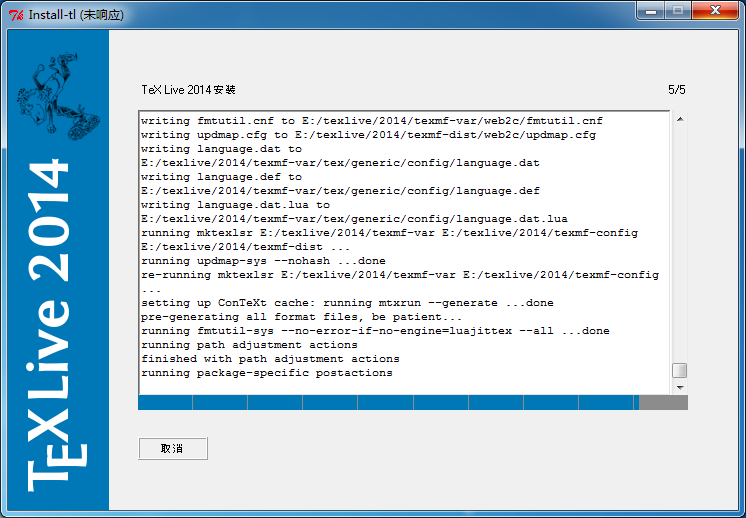
\includegraphics[scale=0.5]{simple8-postinstall.png}
  \end{figure}
\end{frame}

% 安装完成
\begin{frame}
  \begin{figure}[h]
  \centering
  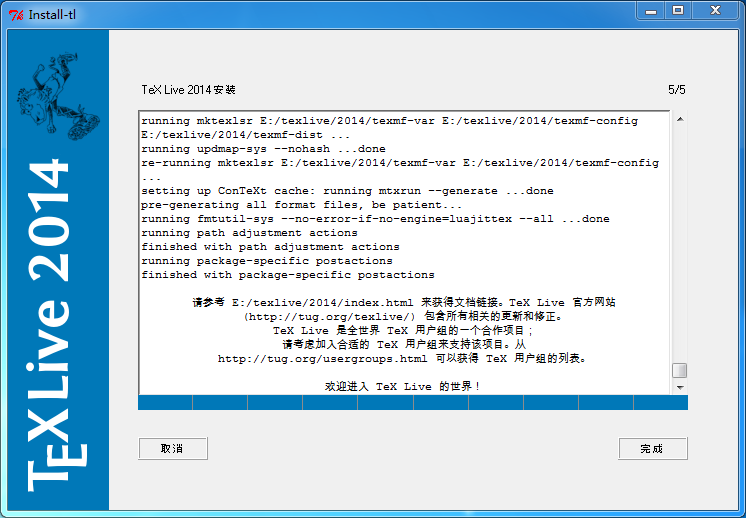
\includegraphics[width=.5\textwidth]{simple9-installed.png}%
  \hspace{2em}
  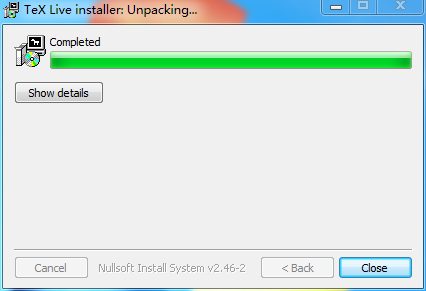
\includegraphics[width=.3\textwidth]{simple10-close.png}
  \end{figure}
\end{frame}

\begin{frame}[fragile]
  \frametitle{网络安装后配置(仅 Linux)}
\begin{itemize}
  \item
    添加环境变量到 \nolinkurl{~/.bash_profile} 文件:
    \begin{lstlisting}
export PATH=/usr/local/texlive/2011/bin/x86_64-linux:$PATH
export MANPATH=/usr/local/texlive/2011/texmf/doc/man:$MANPATH
export INFOPATH=/usr/local/texlive/2011/texmf/doc/info:$INFOPATH
    \end{lstlisting}

  \item
打开 \TeXLive 指南中文版 ``texlive-zh-cn.pdf'',
关注第 3.4 节
  \begin{lstlisting}
texdoc texlive-zh
  \end{lstlisting}

\end{itemize}
\end{frame}

\begin{frame}[fragile]
  \frametitle{网络安装后配置(仅 Linux)}
  \begin{itemize}
\item
\XeTeX\ 系统字体配置
\begin{lstlisting}
cp /usr/local/texlive/2011/texmf-var/fonts/conf/texlive-fontconfig.conf /etc/fonts/conf.d/09-texlive.conf
fc-cache -fsv
\end{lstlisting}

\end{itemize}
\end{frame}

\begin{frame}{编辑器配置}
  \begin{itemize}
    \item \TeX{}编辑器
      \begin{itemize}
        \item 专用编辑器:TeXworks、WinEdt 等
        \item 通用编辑器(加 LaTeX 插件):Vim、Emacs 等
      \end{itemize}
  \end{itemize}
  \begin{exampleblock}{TeXworks 配置}
    \begin{itemize}
      \item 菜单:编辑---首选项
        \begin{itemize}
          \item 编辑器:打开行号
          \item 排版:处理工具下方默认 $\Rightarrow$ 选择 XeLaTeX
        \end{itemize}
    \end{itemize}
  \end{exampleblock}
\end{frame}

\lstdefinestyle{latex}{
language={[LaTeX]TeX},
frame=single,
rulecolor=\color{red!75!green!50!blue},
fillcolor=\color{red!75!green!50!blue!15},
escapeinside=``,
%keywordstyle=\color{red!70},
basicstyle=\color{DarkBlue},
}

%\begin{frame}
  %\frametitle{网络安装后测试}
  %\framesubtitle{English 测试}

  %\begin{exampleblock}{使用已安装的示例文件}
    %\begin{itemize}
      %\item \texttt{latex sample2e.tex \#} .tex $\rightarrow$ .dvi (device independent)

      %\texttt{xdvi sample2e.dvi \#} also try dvipdf sample2e.dvi
      %\item try \texttt{pdflatex sample2e} directly
      %\item \texttt{xetex opentype-info.tex \#} test of xetex's OpenType support
    %\end{itemize}

  %\end{exampleblock}
%\end{frame}

\begin{frame}[fragile]
  \frametitle{网络安装后测试}

  \begin{itemize}
    \item 编辑 \texttt{test-chinese.tex} (Windows 下不要用中文文件名)
      \begin{center}
\begin{lstlisting}[style=latex]
\documentclass{ctexart}
\begin{document}
\TeX{}你好!
\end{document}
\end{lstlisting}
      \end{center}
      \begin{itemize}
        \item Windows 下缺省使用中易字体
        \item Linux 下需要自定义字体(nofonts 选项)
      \end{itemize}
    \item 使用 XeLaTeX 引擎编译,得到 PDF 文档
      \begin{center}
      \fbox{\textrm \TeX{}\songti 你好!}
      \end{center}
  \end{itemize}
\end{frame}

\section{学术论文排版}
\subsection{论文模板使用}

\begin{frame}{模板是什么?}
  \begin{itemize}
    \item 模板
      \begin{itemize}
        \item 已经设计好的格式框架
        \item 好的模板:使用户专注于内容
        \item 不应将时间花费在调整框架上
      \end{itemize}
    \item 再提 Office 和 Word
      \begin{itemize}
        \item 很少有人会有意识地在 Word 中使用模板
        \item 定义自己的标题?定义自己的列表?定义自己的段落样式?
        \item 自动化,还是手工调?
        \item 经常被折腾的精疲力竭
        \item 写论文成了学习 WORD,大量不必要的精力消耗
      \end{itemize}
  \end{itemize}
\end{frame}

\begin{frame}{论文排版}
  \begin{itemize}
    \item 获取模板
      \begin{itemize}
        \item 随发行版自带、手动网络下载
        \item 模板文档类 .cls 文件
        \item 示例 .tex 文件
      \end{itemize}
    \item 编辑 .tex 文件:添加用户内容
    \item 编译:生成 PDF 文档
  \end{itemize}
\end{frame}

\begin{frame}[fragile]{论文排版举例}
  \begin{exampleblock}{IEEE 期刊论文}
    \begin{itemize}
      \item 获取模板:已随发行版自带
        \begin{itemize}
          \item 在安装目录 \lstinline|<prefix>\texlive\2014\|
            下搜索 \lstinline|bare_jrnl.tex|
        \end{itemize}
      \item 编辑 .tex 文件
        \begin{itemize}
          \item 打开 \lstinline|bare_jrnl.tex|,另存到个人论文存放的文件夹
        \end{itemize}
      \item 编译
        \begin{itemize}
          \item 英文文献:XeLaTeX、PDFLaTeX 编译均可
        \end{itemize}
    \end{itemize}
  \end{exampleblock}
\end{frame}

\subsection{\LaTeX{}常用命令}

\begin{frame}[fragile]{\LaTeX{}命令}
  \framesubtitle{\emph{宏} (Macro)、或者\emph{控制序列} (control sequence)}
\begin{itemize}
\item 简单命令
  \begin{itemize}
    \item \verb|\命令|\hspace{2em}
    \verb|{\songti 中国人民解放军}| ~$\Rightarrow$ {\songti 中国人民解放军}
  \item \verb|\命令[可选参数]{必选参数}|\\
\verb|section[精简标题]}{这个题目实在太长了放到目录里面不太好看|\\
$\Rightarrow$ {\heiti 1.1 \hspace{1em} \songti 这个题目实在太长了放到目录里面不太好看}
  \end{itemize}
\item 环境
  \begin{columns}[c]
  \begin{column}{0.45\textwidth}
\begin{lstlisting}[style=latex]
\begin{equation*}
  a^2-b^2=(a+b)(a-b)
\end{equation*}
\end{lstlisting}
\end{column}\hspace{1em}
  \begin{column}{0.45\textwidth}
$ a^2-b^2=(a+b)(a-b)$
\end{column}
  \end{columns}
\end{itemize}
\end{frame}

\begin{frame}[fragile]{\LaTeX{} 常用命令}
  \begin{exampleblock}{命令}
\centering
\footnotesize
  \begin{tabular}{llll}
    \cmd{chapter} & \cmd{section} & \cmd{subsection} & \cmd{paragraph} \\
    章 & 节 & 小节 & 带题头段落 \\\hline
    \cmd{centering} & \cmd{emph} & \cmd{verb} & \cmd{url} \\
   居中对齐         &  强调      & 原样输出   & 超链接 \\\hline
  \cmd{footnote} & \cmd{item} & \cmd{caption} & \cmd{includegraphics} \\
   脚注 & 列表条目 & 标题 & 插入图片 \\\hline
  \cmd{label} & \cmd{cite} & \cmd{ref} \\
  标号 & 引用参考文献 & 引用图表公式等\\\hline
  \end{tabular}
\end{exampleblock}
\end{frame}
\begin{frame}[fragile]{\LaTeX{} 常用命令}
\begin{exampleblock}{环境}
\centering
\footnotesize
\begin{tabular}{lll}
  \env{table} & \env{figure} & \env{equation}\\
  表格 & 图片 & 公式 \\\hline
  \env{itemize} & \env{enumerate} & \env{description}\\
  无编号列表 & 编号列表 & 描述 \\\hline
\end{tabular}
\end{exampleblock}
\end{frame}

\begin{frame}{\LaTeX{}命令举例}
\cmdxmp{chapter}{前言}{\heiti 第 1 章\hspace{1em} 前言}
\cmdxmp{section[精简标题]}{这个题目实在太长了放到目录里面不太好看}{\heiti 1.1
  \hspace{1em} 这个题目实在太长了放到目录里面不太好看}
\cmdxmp{footnote}{我是可爱的脚注}{前方高能\footnote{我是可爱的脚注}}
\end{frame}

\begin{frame}[fragile]{\LaTeX{} 环境命令举例}
  \begin{minipage}{0.4\linewidth}
\begin{lstlisting}[style=latex]
\begin{itemize}
  \item 一条
  \item 次条
  \item 再条
\end{itemize}
\end{lstlisting}
  \end{minipage}\hspace{1.5cm}
  \begin{minipage}{0.4\linewidth}
\begin{itemize}
  \item 一条
  \item 次条
  \item 再条
\end{itemize}
  \end{minipage}
\medskip

  \begin{minipage}{0.4\linewidth}
\begin{lstlisting}[style=latex]
\begin{enumerate}
  \item 一条
  \item 次条
  \item 再条
\end{enumerate}
\end{lstlisting}
  \end{minipage}\hspace{1.5cm}
  \begin{minipage}{0.4\linewidth}
\begin{enumerate}
  \item 一条
  \item 次条
  \item 再条
\end{enumerate}
  \end{minipage}
\end{frame}

\begin{frame}[fragile]{自动引用举例}
  \begin{itemize}
  \item 给对象命名:图片、表格、公式等\\
  \verb|\label{name}|
\item 引用对象\\
  \verb|\ref{name}|
  \end{itemize}
\bigskip

  \begin{minipage}{0.5\linewidth}
\begin{lstlisting}[style=latex,basicstyle=\tiny]
图书馆馆徽请参见图~\ref{fig:lib}。
\begin{figure}
  \centering
  \includegraphics[height=0.2\textheight]%
  {libicon.jpg}
  \caption{图书馆馆徽。}
  \label{fig:lib}
\end{figure}
\end{lstlisting}
  \end{minipage}\hfill
  \begin{minipage}{0.4\linewidth}\centering
    {\songti 图书馆馆徽请参见图~1。}\\[1em]
 
\includegraphics[height=0.2\textheight]{libicon.jpg}\\
 {\footnotesize\heiti 图~1. 图书馆馆徽。}
  \end{minipage}
\end{frame}

\begin{frame}[fragile]{自动引用举例}
\begin{minipage}{0.5\linewidth}
  \begin{lstlisting}[style=latex,basicstyle=\tiny]
\begin{table}
   \centering
   \begin{tabular}{ll}\hline
     编号 & 含义 \\\hline
     1    & 第一 \\
     2    & 第二 \\\hline
   \end{tabular}
   \caption{编号与含义。}
   \label{tab:number}
\end{table}
编号与含义请参见表~\ref{tab:number}。
\end{lstlisting}
\end{minipage}
\begin{minipage}{0.4\linewidth}
\centering\small
 \begin{tabular}{ll}\hline
编号 & 含义 \\\hline
1 & 第一\\
2  & 第二\\\hline
\end{tabular}\\[5pt]
{\small 表~1. 编号与含义}\\[1em]
\normalsize 编号与含义请参见表~1。
\end{minipage}
\end{frame}

\section{学位论文排版}
\subsection{\ThuThesis 清华大学学位论文模板}

\begin{frame}{\ThuThesis}
  \framesubtitle{清华大学学位论文 \LaTeX{} 模板}
  \begin{itemize}
  \item 最早:王磊~(2004.4)
  \item 2005 年:薛瑞尼
  \item 最新发布版:\ThuThesis v4.8.1 (2014/12/09)
  \item 全面支持本科、硕士、博士、博士后论文格式
  \end{itemize}
  \begin{figure}[htbp]
    \centering
    
\includegraphics[height=.4\textheight]{cover-bachelor-crop.pdf}\hfill
    
\includegraphics[height=.4\textheight]{cover-master-crop.pdf}\hfill
    
\includegraphics[height=.4\textheight]{cover-doctor-crop.pdf}\hfill
    
\includegraphics[height=.4\textheight]{cover-postdoctor-crop.pdf}
  \end{figure}
\end{frame}

\begin{frame}{安装\ThuThesis}
  \framesubtitle{以开发版本为例}
      \begin{columns}
        \begin{column}{.7\textwidth}
  \begin{itemize}
    \item 下载最新版
      \begin{itemize}
        \item \url{https://github.com/xueruini/thuthesis}
        \item 右边栏
          \href{https://github.com/xueruini/thuthesis/archive/master.zip}%
          {Download ZIP} 按钮
        \item Git 用户还可以直接克隆仓库
      \end{itemize}
  \end{itemize}
        \end{column}
        \begin{column}{.3\textwidth}
          \begin{figure}[htbp]
            \centering
            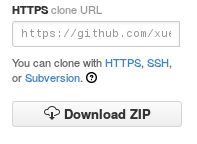
\includegraphics[width=\textwidth]{thuthesis-download.png}
          \end{figure}
        \end{column}
      \end{columns}
  \begin{itemize}
    \item 安装
      \begin{itemize}
        \item 解压缩看文档 \texttt{README.md}
        \item 模板文档类:latex 引擎处理 \texttt{thuthesis.ins} $\Rightarrow$
          \texttt{thuthesis.cls} 和 \texttt{thuthesis.cfg}
        \item 用户手册:latexmk 处理 \texttt{thuthesis.dtx} $\Rightarrow$
          \texttt{thuthesis.pdf}
        \item 论文示例:latexmk 处理 \texttt{main.tex} $\Rightarrow$ \texttt{main.pdf}
        \item 提供有 Makefile 自动化上述过程
      \end{itemize}
  \end{itemize}
\end{frame}

\begin{frame}[fragile]{论文选项}
\begin{description}
\item[bachelor] 我要写本科论文
  \begin{lstlisting}
\documentclass[bachelor]{thuthesis}
  \end{lstlisting}
\item[master] 我要写硕士论文
  \begin{lstlisting}
\documentclass[master]{thuthesis}
  \end{lstlisting}
\item[doctor] 我要写博士论文
  \begin{lstlisting}
\documentclass[doctor]{thuthesis}
  \end{lstlisting}
\item[secret] 论文有保密要求
  \begin{lstlisting}
\documentclass[doctor, secret]{thuthesis}
\secretlevel{机密}
\secretyear{2010}
  \end{lstlisting}
\end{description}
\end{frame}

\begin{frame}{封面}
  \begin{table}[h]
    \centering
\footnotesize
  \begin{tabular}{lll}
    命令作用 & 中文命令 & 英文命令 \\\hline\hline
  论文标题 & \cmd{ctitle} &\cmd{etitle}\\
  作者姓名&  \cmd{cauthor} &\cmd{eauthor}\\
  申请学位名称 & \cmd{cdegree}&\cmd{edegree}\\
  院系名称 & \cmd{cdepartment} & \cmd{edepartment}\\
  专业名称 & \cmd{cmajor} & \cmd{emajor}\\
  导师 & \cmd{csupervisor} & \cmd{esupervisor}\\
  副导师 & \cmd{cassosupervisor} & \cmd{eassosupervisor}\\
  联合导师 & \cmd{ccosupervisor} & \cmd{ecosupervisor}\\
  日期 & \cmd{cdate} & \cmd{edate}\\
  摘要 & \cmd{cabstract} & \cmd{eabstract}\\
  关键词 & \cmd{ckeywords} & \cmd{ekeywords}\\\hline
  \end{tabular}
  \end{table}
\end{frame}

\begin{frame}{数学}
  \begin{itemize}
    \item 公式示例:\nolinkurl{data/chap01.tex}
    \item \ThuThesis{} 定义了常用的数学环境
      \begin{table}[h]
        \centering
    \begin{tabular}{lllll}\hline
axiom & theorem & definition & proposition & lemma \\
公理 & 定理 & 定义 & 命题 & 引理 \\\hline
proof & corollary & example & exercise &\\
证明 & 推论 & 例子& 练习 &\\\hline
    \end{tabular}
      \end{table}
  \end{itemize}
\end{frame}

\begin{frame}[fragile,]{参考文献}
  \begin{itemize}
    \item 推荐 \BibTeX
      \begin{itemize}
        \item 参考文献管理自动化
        \item bib 文件
        \item bst 参考文献样式文件:thubib.bst
      \end{itemize}
    \item 学校要求两种引用方式:
      \begin{itemize}
        \item 上标模式:如``在许多文献$^{[12,13]}$中……''
        \begin{lstlisting}
  \cite{key12, key13}
        \end{lstlisting}
      \item 正文模式:如``文献~[14] 证明了……''
        \begin{lstlisting}
  \onlinecite{key14}
        \end{lstlisting}
      \end{itemize}
    \end{itemize}
\end{frame}

\begin{frame}{作图}
  \begin{columns}[c]
    \begin{column}{.5\textwidth}
  \begin{itemize}
  \item 矢量图 eps, ps, pdf
    \begin{itemize}
    \item \MP, pstricks, pgf $\ldots$
    \item Xfig, Dia, Visio, Inkscape $\ldots$
    \end{itemize}
  \item 标量图 png, jpg, tiff $\ldots$
    \begin{itemize}
      \item 提高清晰度,避免发虚
    \end{itemize}
  \item 转化
    \begin{itemize}
    \item 虚拟打印机
    \item ImageMagick
    \item epstopdf
    \item pdfcrop
    \end{itemize}
  \end{itemize}
    \end{column}
    \begin{column}{.4\textwidth}
\begin{figure}[h]
  \centering
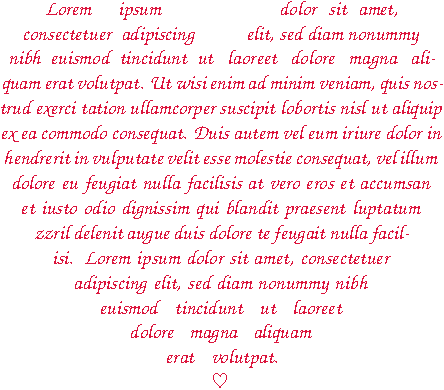
\includegraphics[height=.3\textheight]{shapepar.pdf}\\\vspace{1cm}
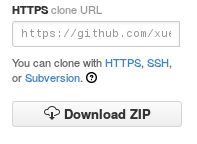
\includegraphics[height=.3\textheight]{thuthesis-download.png}
\end{figure}
    \end{column}
  \end{columns}
\end{frame}

\section{总结}

\begin{frame}{常见问题}
  \begin{itemize}
  \item \alert{编译不通过} 缺少必要宏包,命令拼写错误,括号未配对等
  \item \alert{表格图片乱跑} \LaTeX{} 自身的浮动定位算法
  \item \alert{段落间距变大} \LaTeX{} 排版算法
  \item \alert{参考文献} 推荐使用 \BibTeX{},也可以手写 \cmd{bibitem}
  \end{itemize}
\end{frame}

\begin{frame}{一点建议}
  \begin{itemize}
    \item 先学习
      \begin{itemize}
        \item 仔细阅读《一份不太简短的~\LaTeXe{} 介绍》(lshort-zh)~(1--2 天)
        \item 粗略阅读《\LaTeXe{} 插图指南》~(2--3 小时)
        \item 仔细阅读《\ThuThesis{} 用户手册》~(20 分钟)
        \item 从~\ThuThesis{} 示例文档入手
      \end{itemize}
  \end{itemize}
\end{frame}

\begin{frame}{利用文档}
  \begin{itemize}
    \item 常用文档
      \begin{itemize}
        \item symbols: 符号大全
        \item Mathmode: 数学参考
        \item ctex, xeCJK: 中文支持
        \item texlive-zh: \TL 安装与使用
        \item 所用宏包文档
      \end{itemize}
    \item 工具
      \begin{itemize}
        \item tlmgr: \TL 管理器
        \item texdoc: \TeX{} 文档查看器\\
          例如:\texttt{texdoc lshort-zh}
      \end{itemize}
  \end{itemize}
\end{frame}

% 寻求帮助
\begin{frame}{求助}
  \begin{columns}[c]
    \begin{column}{.45\textwidth}
      \begin{itemize}
        \item BBS
          \begin{itemize}
            \item \href{http://www.newsmth.net/nForum/board/TeX}{水木
              社区 TeX 版}
            \item \href{http://bbs.ctex.org/}{bbs.ctex.org}
          \end{itemize}
        \item \href{http://www.tex.ac.uk/cgi-bin/texfaq2html}{UK FAQ}
        \item TeX StackExchange
        \item \href{http://justfuckinggoogleit.com/}{Google}
      \end{itemize}
    \end{column}
    \begin{column}{.45\textwidth}
      
\includegraphics[width=\textwidth]{TFZsuperellipse-crop.pdf}
    \end{column}
  \end{columns}
\end{frame}

\begin{frame}{\ThuThesis 问题}
\begin{itemize}
\item GitHub Issues 提问
\item \TeX @newsmth 查找或发文
\item \href{http://groups.google.com/group/thuthesis}\ThuThesis{} Google Group 发问
\end{itemize}
\end{frame}


\begin{frame}{你也可以帮助}
\begin{itemize}
\item 错误反馈:GitHub Issues
\item 改进建议:GitHub Issues
\item 出力维护:LaTeX 宏包编写、Git
\item 科普、答疑\pause \hspace{2em}\alert{图书馆讲座征主讲人!}
\end{itemize}
\end{frame}

\section*{附录}

\begin{frame}
  \begin{itemize}
    \item 本幻灯片:\url{https://github.com/alick/thulib-latex-talk}
    \item 本幻灯片基于:
      \begin{itemize}
        \item \url{http://github.com/alick/fad-texlive-talk}
        \item \ThuThesis{}使用向导 v3.0
      \end{itemize}
    \item 许可证:CC BY-SA 4.0 Unported \cc\ccby\ccsa
  \end{itemize}
\end{frame}

\begin{frame}{扩展阅读}
  \begin{itemize}
    \item \LaTeX\ Tips:
      \url{https://alick.fedorapeople.org/fudcon-apac-2014/latex-tips.pdf} \\
      (例如:\LaTeX{} 中引号的正确输入姿势)
    \item Linux 用户:\url{https://github.com/alick/fad-texlive-talk}
    \item \ThuThesis{}使用向导 v3.0 (薛瑞尼)
    \item \LaTeX{}杂谈(刘海洋)
    \item 《\LaTeX{}入门》(刘海洋)
  \end{itemize}
\end{frame}

\begin{frame}{\LaTeX{}讲座预告}
  \begin{itemize}
    \item \TeX{} 与汉字处理
      \begin{itemize}
        \item 主讲人:马起园、刘海洋
        \item 主办:清华 TUNA 协会
        \item 时间:暂定下月
        \item 地点:校内
      \end{itemize}
  \end{itemize}
\end{frame}

\begin{frame}
  \begin{center}
    {\Huge\calligra Thank you!}
  \end{center}
  \begin{figure}[htbp]
    \centering
    
\includegraphics[height=.2\textheight]{url.pdf}
  \end{figure}
\end{frame}

\end{document}
%%% vim: set sw=2 isk+=\: et tw=80 cc=+1 formatoptions+=mM:
